
\section{Resultados}

O treinamento da rede de classificação se deu em 10 segundos. O treinamento foi
interrompido por se atingir limite inferior do gradiente (múltiplas execuções).

A rede neural classificou corretamente todas as amostras (figura
\ref{Figure-031-ConfusionMatrix}) em intervalo de tempo aproximado de 1 segundo.
Apesar de a rede classificar as amostras, não existe associação útil entre o
número da classe e o indivíduo correspondente.

\begin{figure*}
  \centering
  \captionsetup{type=figure}
  \hspace*{-12cm}
  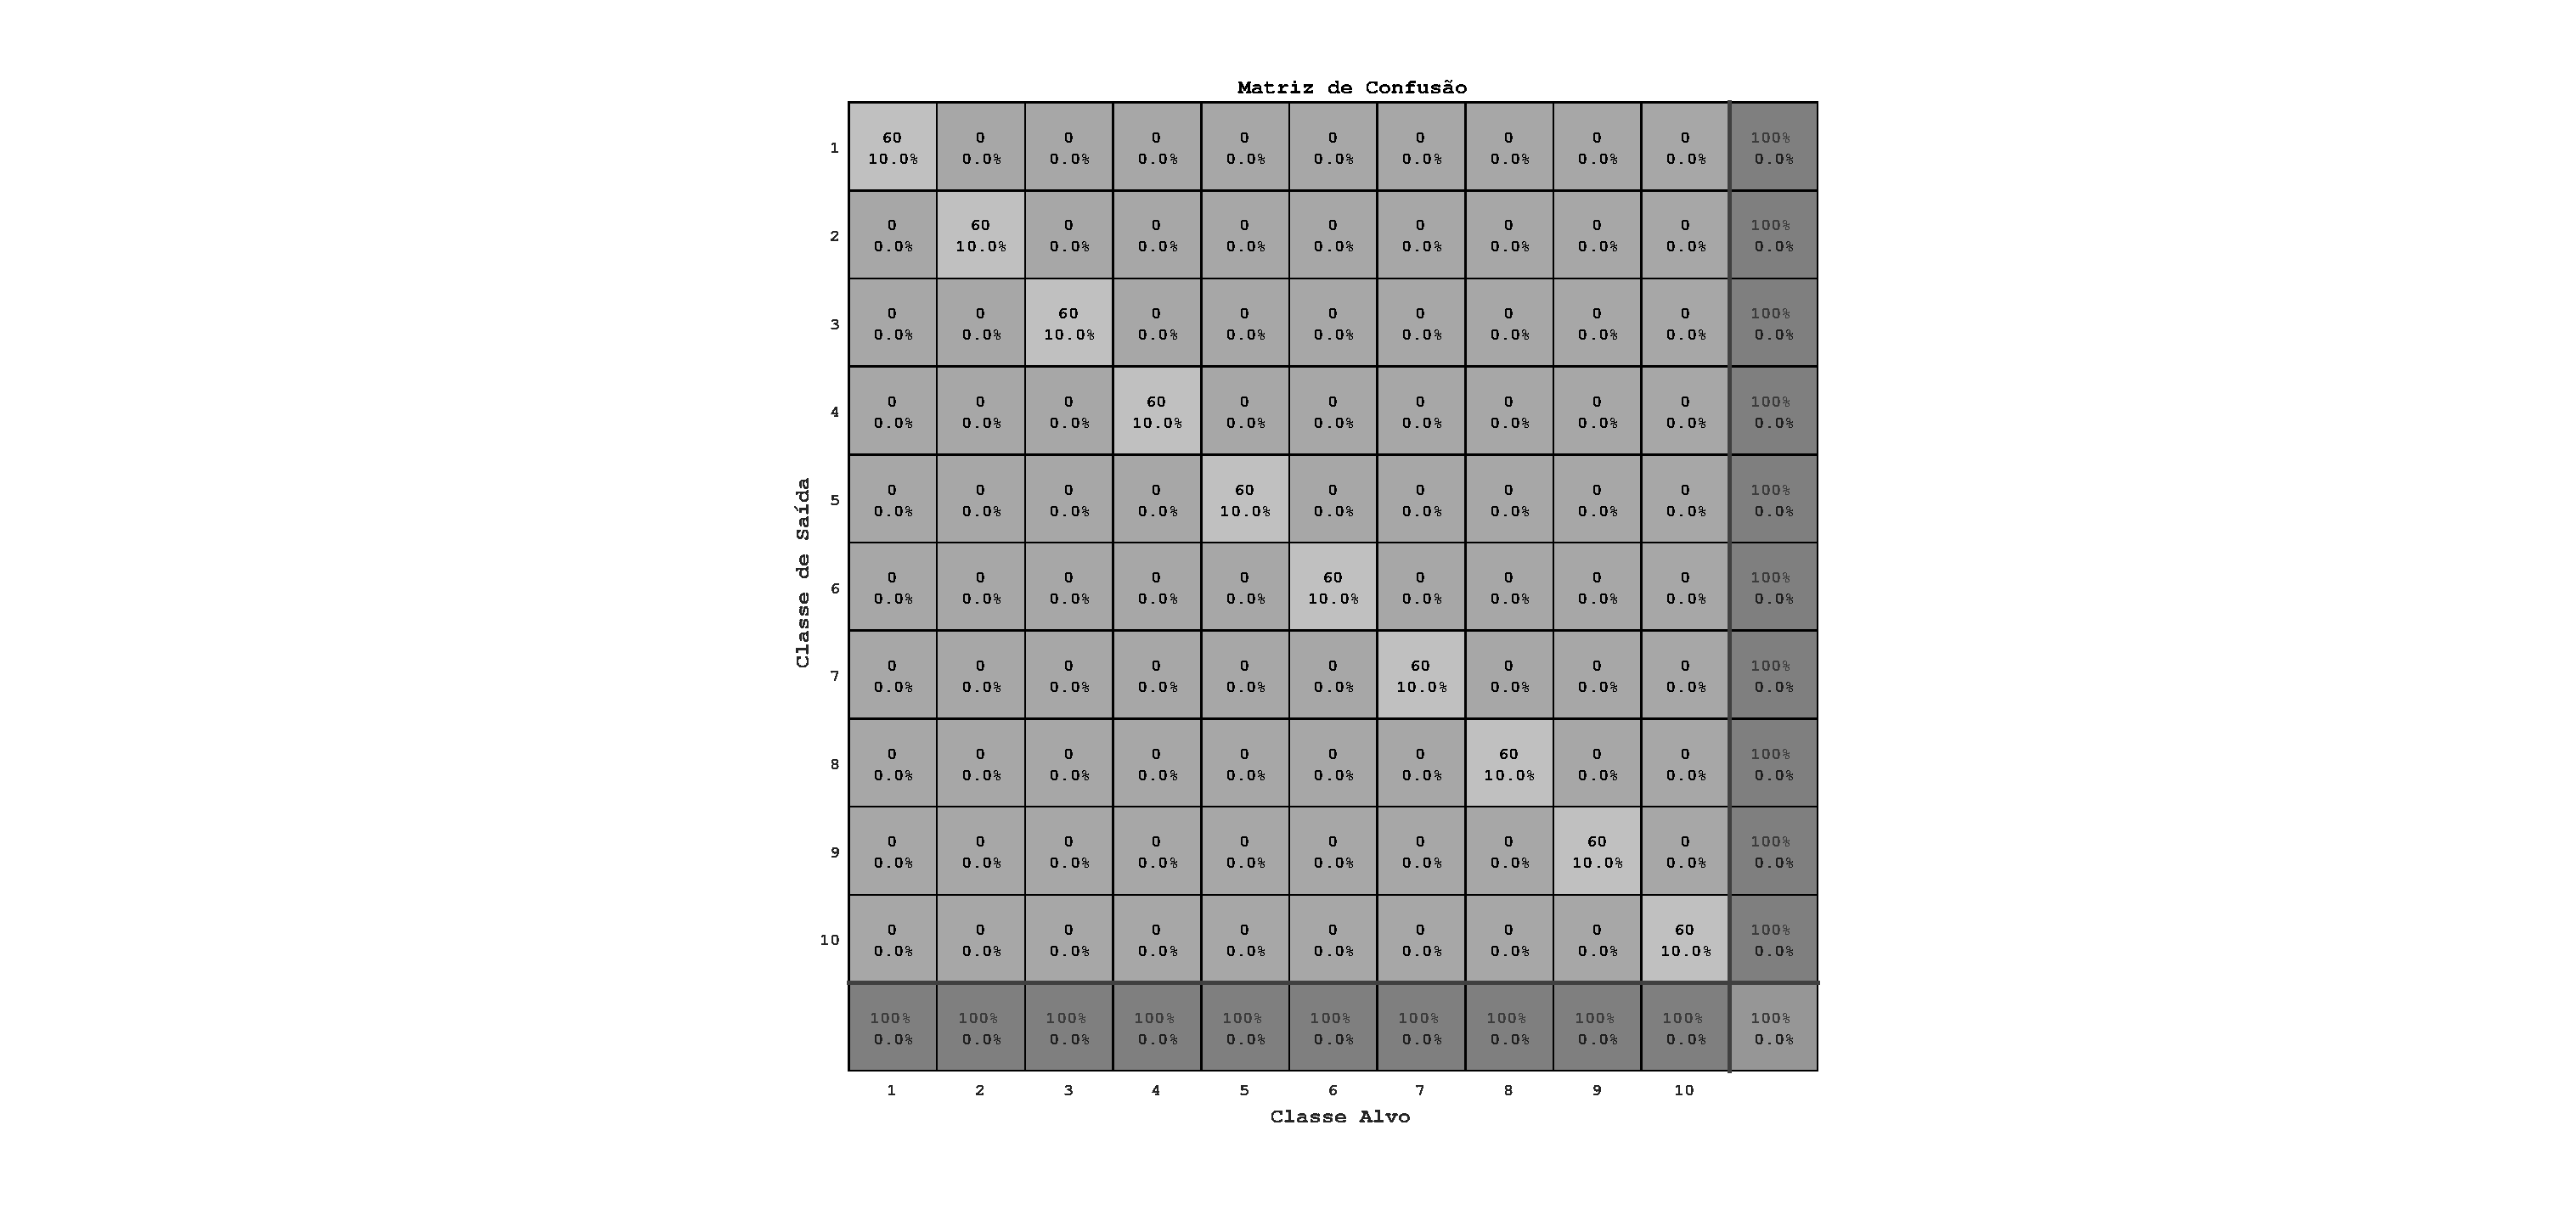
\includegraphics[scale=0.75]{./figures/Figure-031-ConfusionMatrix.eps}
  \captionof{figure}{
    Matriz de confusão. A rede classificou corretamente todas as amostras. Cada
    classe tem 60 amostras correspondentes.
    \hfill \break
  }
	\label{Figure-031-ConfusionMatrix}
\end{figure*}

\begin{figure*}
  \centering
  \captionsetup{type=figure}
  \hspace*{-1.75cm}
  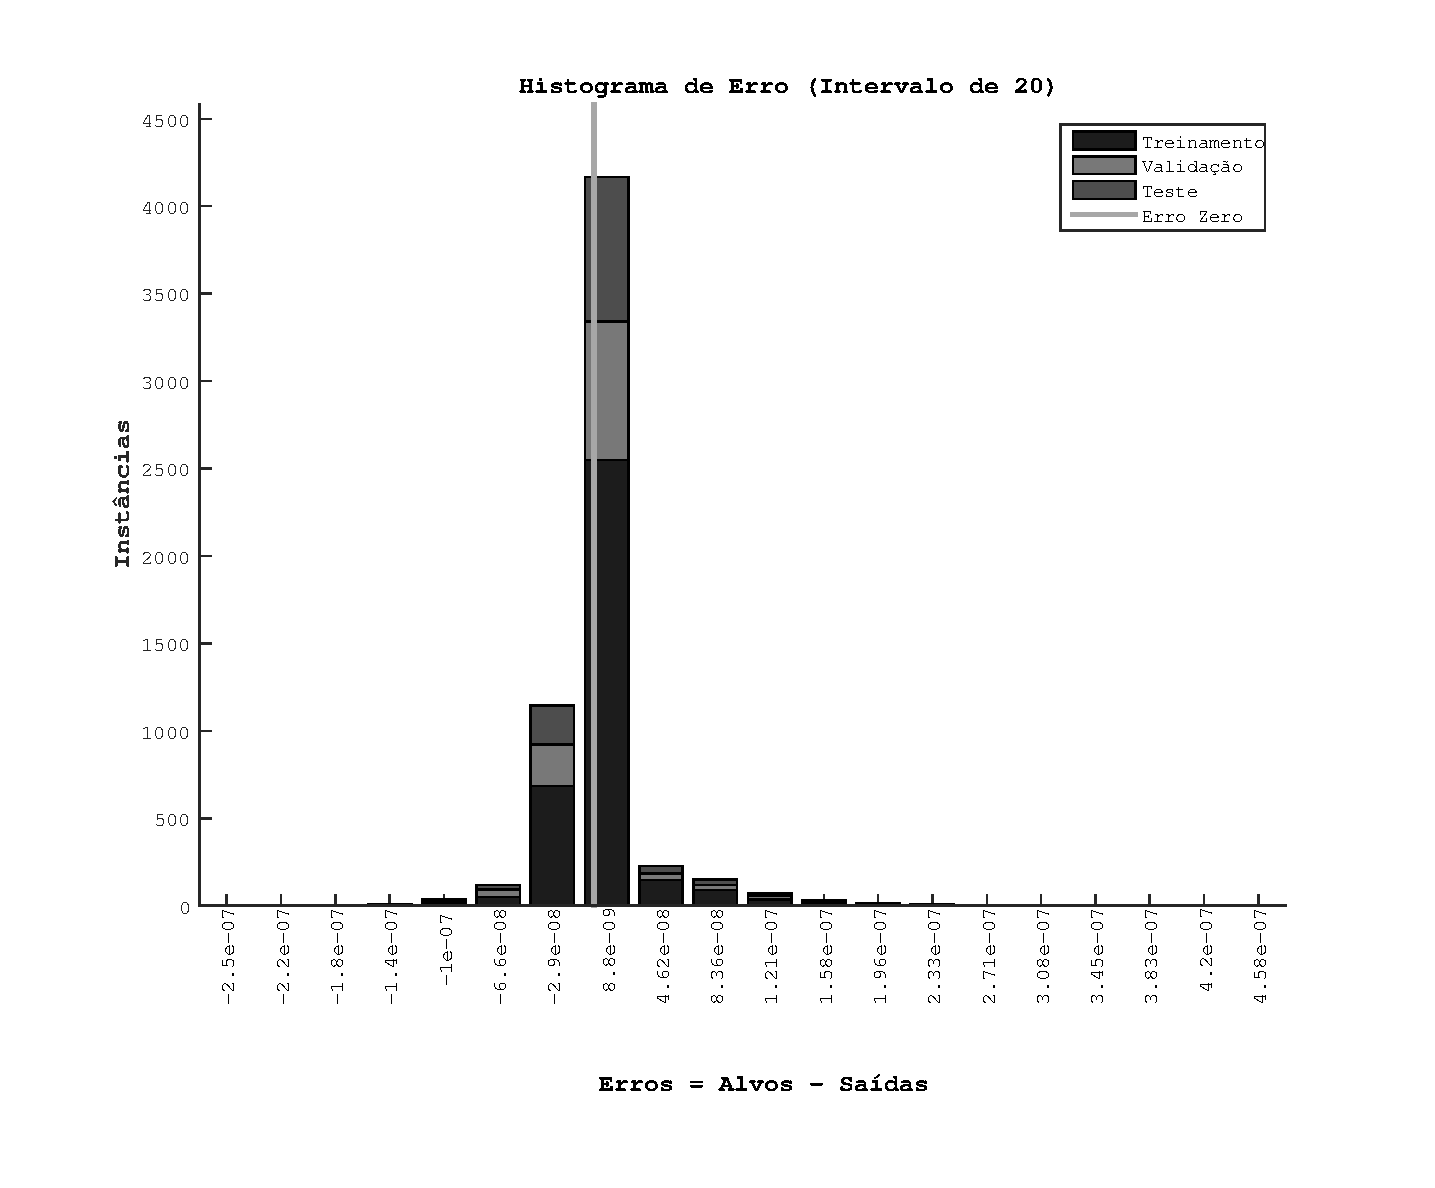
\includegraphics[scale=0.8]{./figures/Figure-032-ErrorHistogram.eps}
  \captionof{figure}{
    Histograma de erro (intervalo de largura 20).
    \hfill \break
  }
	\label{Figure-032-ErrorHistogram}
\end{figure*}

\begin{figure*}
  \centering
  \captionsetup{type=figure}
  \hspace*{-1.75cm}
  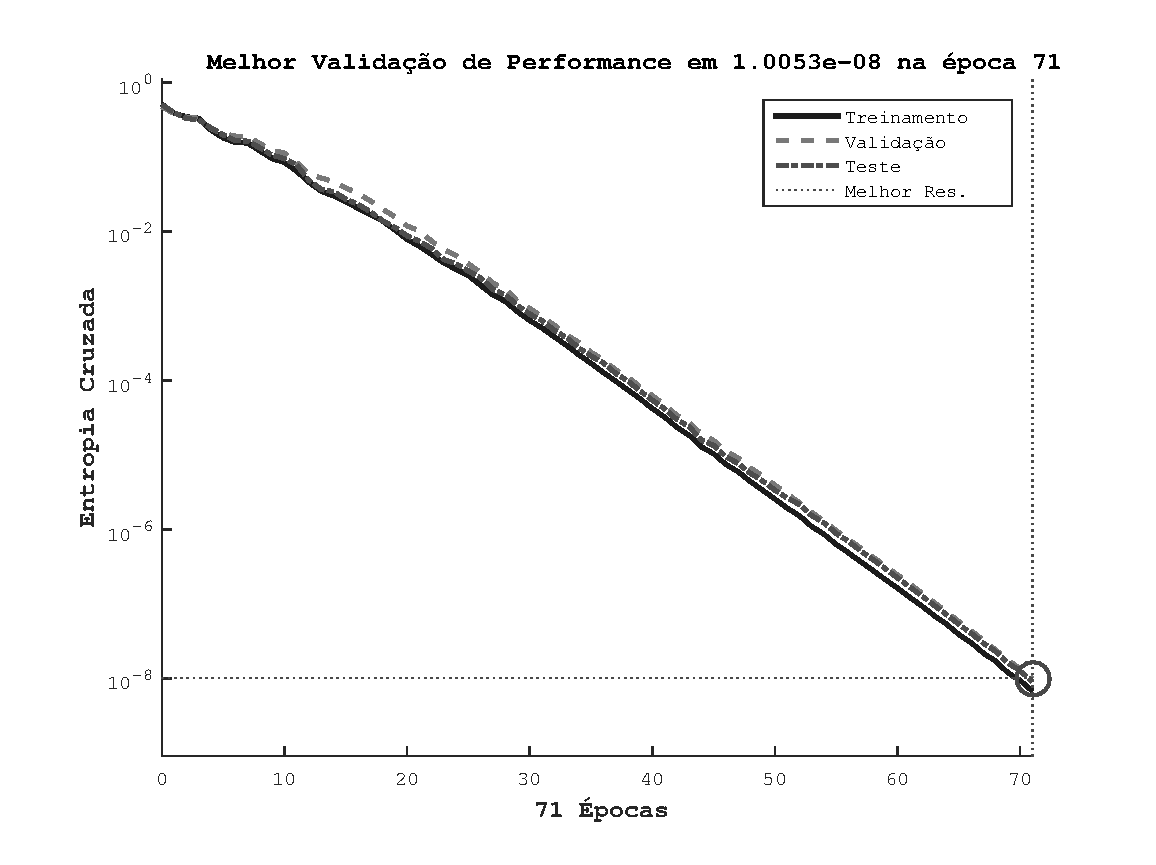
\includegraphics[scale=0.625]{./figures/Figure-033-Performance.eps}
  \captionof{figure}{
    Evolução da entropia cruzada por épocas de treinamento. Apesar do
    decrescimento aproximadamente linear, o treinamento foi interrompido com
    finalidade de se evitar \textit{overfitting}.
    \hfill \break
  }
	\label{Figure-033-Performance}
\end{figure*}

\begin{figure*}
  \centering
  \captionsetup{type=figure}
  \hspace*{-1.75cm}
  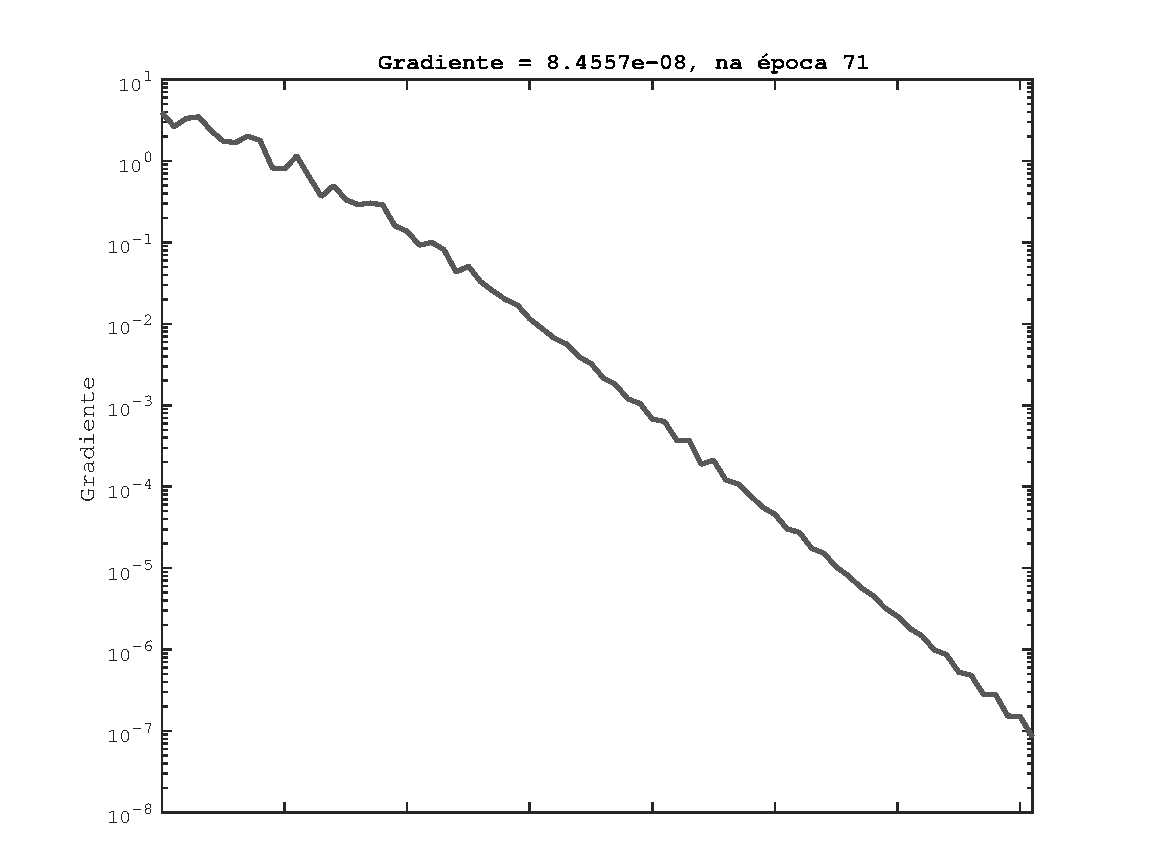
\includegraphics[scale=0.625]{./figures/Figure-034-Gradient.eps}
  \captionof{figure}{
    Evolução do gradiente por épocas de treinamento. Apesar do decrescimento
    logarítmico, o treinamento foi interrompido com finalidade de se evitar
    \textit{overfitting}.
    \hfill \break
  }
	\label{Figure-034-Gradient}
\end{figure*}

A performance e o gradiente de treinamento decaem rapidamente (figuras
\ref{Figure-033-Performance} e \ref{Figure-034-Gradient}), mas, com o limiar
inferior do gradiente atingido, o treinamento é interrompido com finalidade de
se evitar \textit{overfitting}. O histograma de erro (figura
\ref{Figure-032-ErrorHistogram}) e a correta classificação das amostras (figura
\ref{Figure-031-ConfusionMatrix}) indicam que a aplicação de uma rede de
classificação se mostrou adequada para resolver o problema de reconhecimento de
locutor.
